\documentclass[letterpaper, 24pt, final, onecolumn, titlepage] {article}

\usepackage{enumerate}
\usepackage{graphicx}
\usepackage{listings}
\usepackage{color}
\usepackage{setspace}
\usepackage {amsmath}
\usepackage{amssymb}
\usepackage{afterpage}
\usepackage{geometry}
\geometry{
 a4paper,
 total={170mm,257mm},
 left=1.5cm,
 right=1.5cm,
}
\title{ECE 270: Computer Methods in ECE \\
	\vspace{1.5cm}
   		\begin{center}\includegraphics{umlogo} \end{center}
	\vspace{1.5cm}
	\textbf{Final Project} \\
	Customize My Ride}
	
\author{Hussein El-Souri}

\date{\today}

\definecolor{dkgreen}{rgb}{0,0.6,0}
\definecolor{gray}{rgb}{0.5,0.5,0.5}
\definecolor{mauve}{rgb}{0.58,0,0.82}

\lstset{frame=tb,
  language=C,
  aboveskip=3mm,
  belowskip=3mm,
  showstringspaces=false,
  columns=flexible,
  basicstyle={\small\ttfamily},
  numbers=none,
  numberstyle=\tiny\color{gray},
  keywordstyle=\color{blue},
  commentstyle=\color{dkgreen},
  stringstyle=\color{mauve},
  breaklines=true,
  breakatwhitespace=true,
  tabsize=3
}

\begin{document}

\maketitle

\doublespacing

\section{Statement of the Problem}

My project is a simple project that allows one to cutstomize a car Colot.

\section{Description of Solution}

In this project I used openframework paths to draw the front,back and side "skeleton" of the car such that i designated a function for each of those(frontCar, sideCar, and BackCar respectively).\\
Each of those functions take in a path and draw the "skeleton" according to that path.\\
Four more functions were created for the details in the front,side,and back(frontDetail,sideDetails, and backDetails repectively).\\
A GUI (Graphical User Interface)was created to control which view the user is loking at along with whether or not music is playing.\\
The GUI also controls the color of the car,tires alon with the Entire position both along the X and Y.\\
The project focuses more on pathing and shape creation and that is where the real work is.\\
The sideCar function takes in a path and draws the path along specific certain points.\\
\begin{center}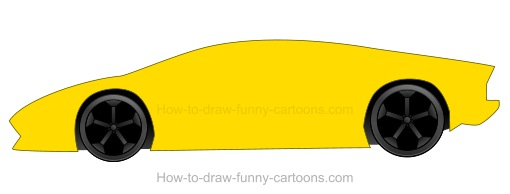
\includegraphics{sideDesign} \end{center}
This picture was used as a "design schematic" or inspiration for my design. Similar to pathing using the pentool on phtotoshop. In fact a bit of photoshop was used to help with the pathing and the pixel designation.\\
For the frontCar function it also takes in a path that follows the design of this picture.\\
\begin{center}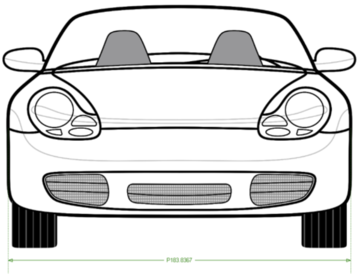
\includegraphics{frontDesign} \end{center}
The backCar is the same as the frontCar but the details are different.\\
and here is where the "details functions" come in. These draw details on the car. Some of these details include doors,handles and windos on the side, windsheild and hood in the front, and wibnsheild and trunk in the back.\\
The path's initiall oisition is ontrolled by a slider through a GUI. The corlors of the tire and car are controlled independantly through another GUI. \\
The Project end result is something very simple; however pathing and shape creation are very difficult and time consuming.\\
\textbf {Please check powerpoint presentation provided with project code in the zip file.}\\



\section{Testing and Output}

\begin{center}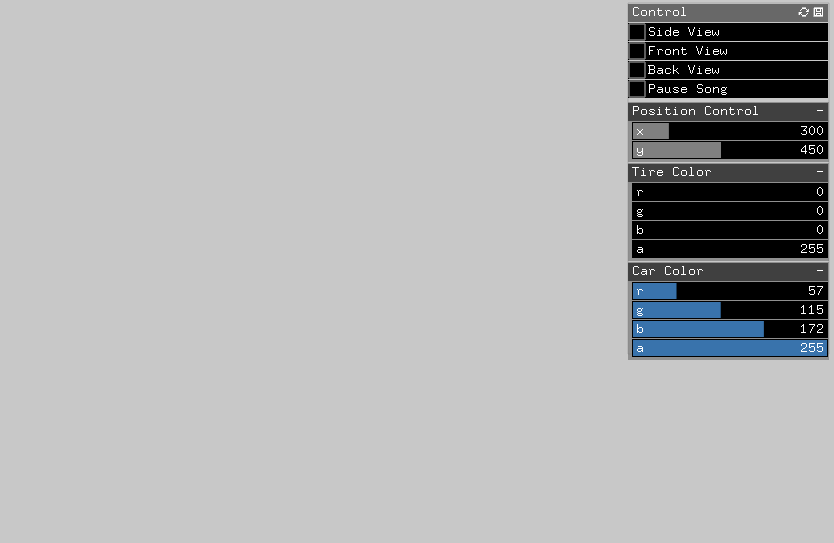
\includegraphics{GUI} \end{center}
\begin{center}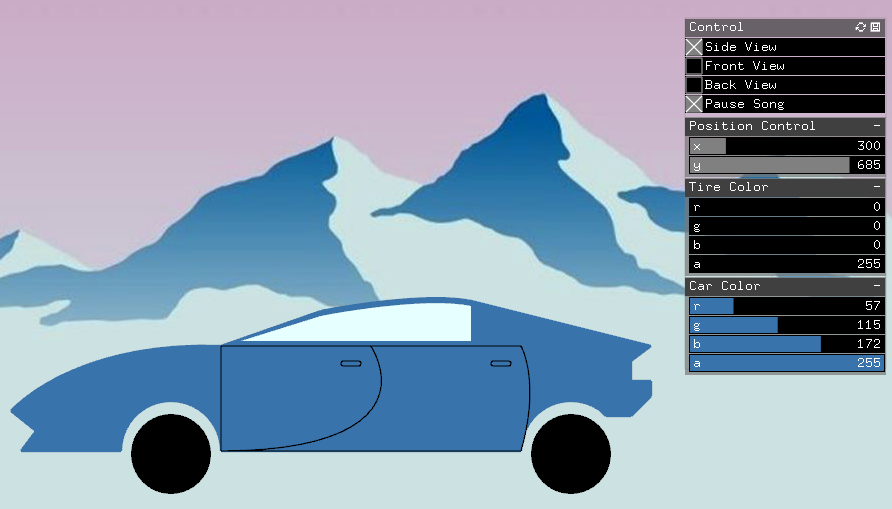
\includegraphics{sideView} \end{center}
\begin{center}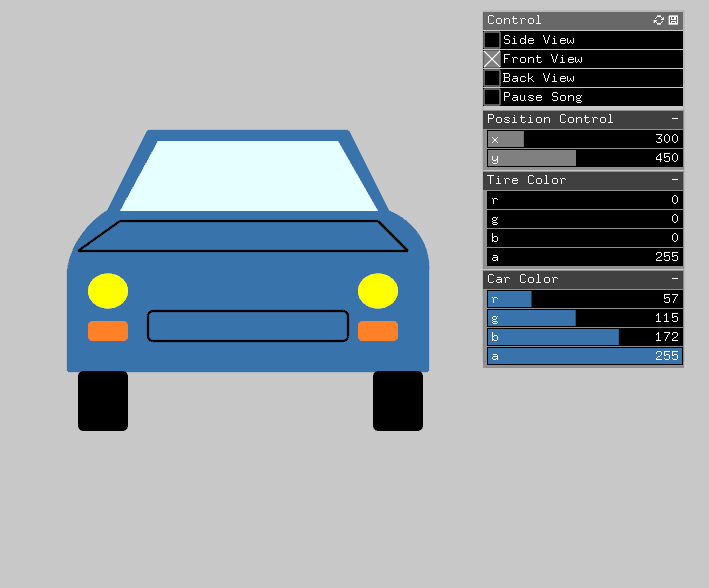
\includegraphics{frontView} \end{center}
\begin{center}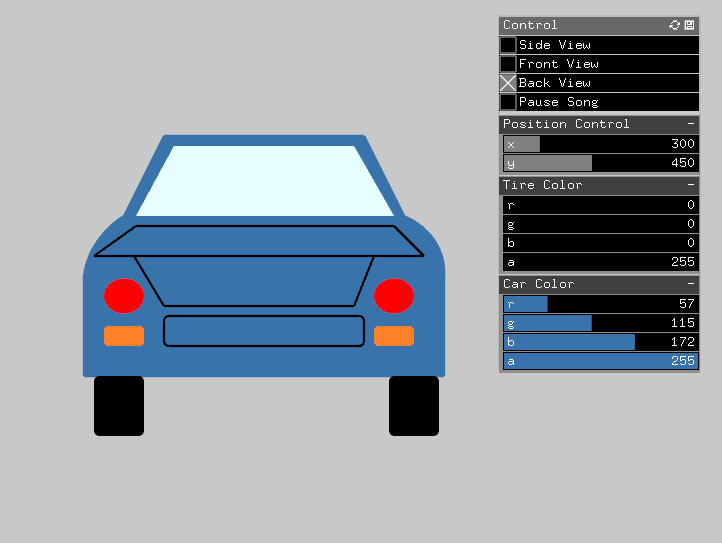
\includegraphics{backView} \end{center}

\pagebreak

\section{Code}
\singlespacing

\begin{lstlisting}

//---ofApp.h

       ofPath sidePath;
        ofPath frontPath;
        ofPath backPath;
        ofVec2f startPos;

		void sideCar(ofPath tempPath);
		void sideDetails();
		//---
		void frontCar(ofPath tempPath);
		void frontDetails();
		//--
		void backCar(ofPath tempPath);
		void backDetails();
		//--
		ofxVec2Slider posControl;
		ofxColorSlider tireColor;
		ofxColorSlider carColor;
		//--
		ofxPanel viewGui;
        ofxToggle sideView;
		ofxToggle frontView;
		ofxToggle backView;
		ofxToggle songPlay;
		//--
		ofSoundPlayer mySong;
//---------------------------------------------------------------------------------------------
//---------------------------------------------------------------------------------------------
//---ofApp.cpp
void ofApp::sideDetails(){

    //---Doors
    ofNoFill();
    ofSetColor(0,0,0);
    ofSetLineWidth(1.5);
    ofBeginShape();
        ofVertex(posControl->x,posControl->y);
        ofVertex(posControl->x,posControl->y-105);
        ofVertex(2*posControl->x,posControl->y-105);
        ofPoint pt1,pt2,pt3;
        pt1.set(2*posControl->x,posControl->y-105);
        pt2.set(2*posControl->x+20,posControl->y-70);
        pt3.set(2*posControl->x,posControl->y);
        ofBezierVertex(pt1,pt2,pt3);
        ofVertex(posControl->x,posControl->y);
        ofPoint pt4,pt5,pt6;
        pt4.set(posControl->x+150,posControl->y);
        pt5.set(posControl->x+180,posControl->y-53);
        pt6.set(posControl->x+150,posControl->y-105);
        ofBezierVertex(pt4,pt5,pt6);
    ofEndShape();
    //---handles
    ofRectRounded(posControl->x+120,posControl->y-90,20,5,20);
    ofRectRounded(posControl->x+270,posControl->y-90,20,5,20);
    //---side windows
    ofSetColor(230, 255, 255);
    ofFill();
    ofBeginShape();
        ofVertex(posControl->x+20,posControl->y-110);
        ofVertex(posControl->x+100,posControl->y-135);
        ofPoint pt7,pt8,pt9;
        pt7.set(posControl->x+100,posControl->y-135);
        pt8.set(posControl->x+200,posControl->y-155);
        pt9.set(posControl->x+250,posControl->y-145);
        ofBezierVertex(pt7,pt8,pt9);
        ofVertex(posControl->x+250,posControl->y-110);
        ofVertex(posControl->x+20,posControl->y-110);
    ofEndShape();

}

void ofApp::sideCar(ofPath tempPath){
    //-- car
    tempPath.setFillColor(carColor);
    tempPath.setStrokeColor(carColor);
    tempPath.setStrokeWidth(2.5);
    tempPath.setArcResolution(200);
    tempPath.moveTo(posControl->x-100,posControl->y);
    tempPath.lineTo(posControl->x-200,posControl->y);
    tempPath.lineTo(posControl->x-185,posControl->y-20);
    tempPath.lineTo(posControl->x-210,posControl->y-40);
    ofPoint pt1,pt2,pt3;
    pt1.set(posControl->x-210,posControl->y-40);
    pt2.set(posControl->x-150,posControl->y-110);
    pt3.set(posControl->x,posControl->y-105);
    tempPath.bezierTo(pt1,pt2,pt3);
    tempPath.lineTo(posControl->x+100,posControl->y-140);
    ofPoint pt4,pt5,pt6;
    pt4.set(posControl->x+100,posControl->y-140);
    pt5.set(posControl->x+200,posControl->y-160);
    pt6.set(posControl->x+250,posControl->y-150);
    tempPath.bezierTo(pt4,pt5,pt6);
    tempPath.lineTo(2*posControl->x+130,posControl->y-105);
    tempPath.lineTo(2*posControl->x+110,posControl->y-90);
    tempPath.lineTo(2*posControl->x+110,posControl->y-70);
    tempPath.lineTo(2*posControl->x+130,posControl->y-70);
    tempPath.lineTo(2*posControl->x+130,posControl->y-55);
    tempPath.lineTo(2*posControl->x+110,posControl->y-35);
    tempPath.lineTo(2*posControl->x+85,posControl->y-35);
    tempPath.arcNegative(2*posControl->x+50,posControl->y,50,50,-55,180);
    tempPath.lineTo(posControl->x,posControl->y);
    tempPath.arcNegative(posControl->x-50,posControl->y,50,50,0,180);
    tempPath.close();
    tempPath.draw();
    //--tires
    ofSetColor(tireColor);
    ofFill();
    ofSetCircleResolution(200);
    ofCircle (posControl->x-50,posControl->y+3,40);
    ofCircle (2*posControl->x+50,posControl->y+3,40);
    sideDetails();

}

void ofApp::frontDetails(){

     //----front bumper
    ofNoFill();
    ofSetColor(0,0,0);
    ofSetLineWidth(2.5);
    ofRectRounded(posControl->x+120,posControl->y-110,200,30,5);
    //----front tires
    ofFill();
    ofSetColor(tireColor);
    ofRectRounded(posControl->x+50,posControl->y-50,50,60,5);
    ofRectRounded(posControl->x+345,posControl->y-50,50,60,5);
    //----front lights
    ofSetColor(255, 255, 0);
    ofEllipse(posControl->x+80,posControl->y-130,40,35);
    ofEllipse(posControl->x+350,posControl->y-130,40,35);
    //----front blinkers
    ofSetColor(255, 128, 38);
    ofRectRounded(posControl->x+60,posControl->y-100,40,20,5);
    ofRectRounded(posControl->x+330,posControl->y-100,40,20,5);
    //--front wind Shield
    ofSetColor(230, 255, 255);
    ofBeginShape();
        ofVertex(posControl->x+350,posControl->y-210);
        ofVertex(posControl->x+310,posControl->y-280);
        ofVertex(posControl->x+130,posControl->y-280);
        ofVertex(posControl->x+92,posControl->y-210);
    ofEndShape();
    //---front hood
    ofNoFill();
    ofSetColor(0,0,0);
    ofBeginShape();
        ofVertex(posControl->x+350,posControl->y-200);
        ofVertex(posControl->x+92,posControl->y-200);
        ofVertex(posControl->x+50,posControl->y-170);
        ofVertex(posControl->x+380,posControl->y-170);
        ofVertex(posControl->x+350,posControl->y-200);
    ofEndShape();


}

void ofApp::frontCar(ofPath tempPath){

    tempPath.setFillColor(carColor);
    tempPath.setStrokeColor(carColor);
    tempPath.setStrokeWidth(2.5);
    tempPath.setArcResolution(200);
    tempPath.moveTo(posControl->x+400,posControl->y-50);
    tempPath.lineTo(posControl->x+400,posControl->y-150);
    ofPoint pt1,pt2,pt3;
    pt1.set(posControl->x+400,posControl->y-150);
    pt2.set(posControl->x+405,posControl->y-190);
    pt3.set(posControl->x+360,posControl->y-210);
    tempPath.bezierTo(pt1,pt2,pt3);
    tempPath.moveTo(pt3);
    tempPath.lineTo(posControl->x+320,posControl->y-290);
    tempPath.lineTo(posControl->x+120,posControl->y-290);
    tempPath.lineTo(posControl->x+80,posControl->y-210);
    ofPoint pt4,pt5,pt6;
    pt4.set(posControl->x+80,posControl->y-210);
    pt5.set(posControl->x+45,posControl->y-190);
    pt6.set(posControl->x+40,posControl->y-150);
    tempPath.bezierTo(pt4,pt5,pt6);
    tempPath.lineTo(posControl->x+40,posControl->y-50);
    tempPath.lineTo(posControl->x+400,posControl->y-50);
    tempPath.moveTo(posControl->x+400,posControl->y-50);
    tempPath.close();
    tempPath.draw();
    frontDetails();
}

void ofApp::backDetails(){


     //----back bumper
    ofNoFill();
    ofSetColor(0,0,0);
    ofSetLineWidth(2.5);
    ofRectRounded(posControl->x+120,posControl->y-110,200,30,5);
    //----back tires
    ofSetColor(tireColor);
    ofFill();
    ofRectRounded(posControl->x+50,posControl->y-50,50,60,5);
    ofRectRounded(posControl->x+345,posControl->y-50,50,60,5);
    //----Back Lights
    ofSetColor(255,0, 0);
    ofEllipse(posControl->x+80,posControl->y-130,40,35);
    ofEllipse(posControl->x+350,posControl->y-130,40,35);
    //----Back Blinkers
    ofSetColor(255, 128, 38);
    ofRectRounded(posControl->x+60,posControl->y-100,40,20,5);
    ofRectRounded(posControl->x+330,posControl->y-100,40,20,5);
    //---back wind shield
    ofSetColor(230, 255, 255);
    ofBeginShape();
        ofVertex(posControl->x+350,posControl->y-210);
        ofVertex(posControl->x+310,posControl->y-280);
        ofVertex(posControl->x+130,posControl->y-280);
        ofVertex(posControl->x+92,posControl->y-210);
    ofEndShape();
    //back trunck
    ofNoFill();
    ofSetColor(0,0,0);
    ofBeginShape();

        ofVertex(posControl->x+350,posControl->y-200);
        ofVertex(posControl->x+92,posControl->y-200);
        ofVertex(posControl->x+50,posControl->y-170);
        ofVertex(posControl->x+380,posControl->y-170);
        ofVertex(posControl->x+350,posControl->y-200);
    ofEndShape();
    ofBeginShape();
        ofVertex(posControl->x+330,posControl->y-170);
        ofVertex(posControl->x+310,posControl->y-120);
        ofVertex(posControl->x+120,posControl->y-120);
        ofVertex(posControl->x+90,posControl->y-170);
    ofEndShape();
}

void ofApp::backCar(ofPath tempPath){

    tempPath.setFillColor(carColor);
    tempPath.setStrokeColor(carColor);
    tempPath.setStrokeWidth(2.5);
    tempPath.setArcResolution(200);
    tempPath.moveTo(posControl->x+400,posControl->y-50);
    tempPath.lineTo(posControl->x+400,posControl->y-150);
    ofPoint pt1,pt2,pt3;
    pt1.set(posControl->x+400,posControl->y-150);
    pt2.set(posControl->x+405,posControl->y-190);
    pt3.set(posControl->x+360,posControl->y-210);
    tempPath.bezierTo(pt1,pt2,pt3);
    tempPath.moveTo(pt3);
    tempPath.lineTo(posControl->x+320,posControl->y-290);
    tempPath.lineTo(posControl->x+120,posControl->y-290);
    tempPath.lineTo(posControl->x+80,posControl->y-210);
    ofPoint pt4,pt5,pt6;
    pt4.set(posControl->x+80,posControl->y-210);
    pt5.set(posControl->x+45,posControl->y-190);
    pt6.set(posControl->x+40,posControl->y-150);
    tempPath.bezierTo(pt4,pt5,pt6);
    tempPath.lineTo(posControl->x+40,posControl->y-50);
    tempPath.lineTo(posControl->x+400,posControl->y-50);
    tempPath.moveTo(posControl->x+400,posControl->y-50);
    tempPath.close();
    tempPath.draw();
    backDetails();
}

//--------------------------------------------------------------
void ofApp::setup(){

    startPos.set(300,450);
    ofSetWindowTitle("Pimp my Ride by Hussein El-Souri");
    //---
    viewGui.setup("Control");
    viewGui.setPosition(900,10);
    viewGui.add(sideView.setup("Side View",false));
    viewGui.add(frontView.setup("Front View",false));
    viewGui.add(backView.setup("Back View",false));
    viewGui.add(songPlay.setup("Pause Song",false));
    viewGui.add(posControl.setup("Position Control",startPos,ofVec2f(210,160),ofVec2f(700,800)));
    viewGui.add(tireColor.setup("Tire Color",ofColor(0,0,0),ofColor(0,0),ofColor(255,255)));
    viewGui.add(carColor.setup("Car Color",ofColor(57, 115, 172),ofColor(0,0),ofColor(255,255)));
    //---
    mySong.loadSound("song.mp3");
    mySong.play();
}

//--------------------------------------------------------------
void ofApp::update(){


}

//--------------------------------------------------------------
void ofApp::draw(){
    viewGui.draw();
    if(songPlay)
    {
        mySong.setPaused(songPlay);
    }
    else
    {
        mySong.setPaused(songPlay);
    }
    if(sideView)
    {
        frontView=false;
        backView=false;
        sideCar(sidePath);

    }
     if(frontView)
    {
        sideView=false;
        backView=false;
        frontCar(frontPath);
    }
    if(backView)
    {
        frontView=false;
        sideView=false;
        backCar(backPath);
    }


}



\end{lstlisting}

\end{document}